\chapter{Kostenplanung}
\label{sec:kostenplanung}

\section{Personalkosten}
Personalkosten entstehen über die Gesamtdauer des Projekts. Um die Kosten eines Arbeitspakets zu ermitteln, ist dessen erwartete Dauer mit dem dazugehörigen Monatslohn und der Anzahl der Personen zu multiplizieren. Die folgende Tabelle zeigt beispielhaft die Berechnung am Arbeitspaket 1: 

\begin{figure}[ht]
	\centering
	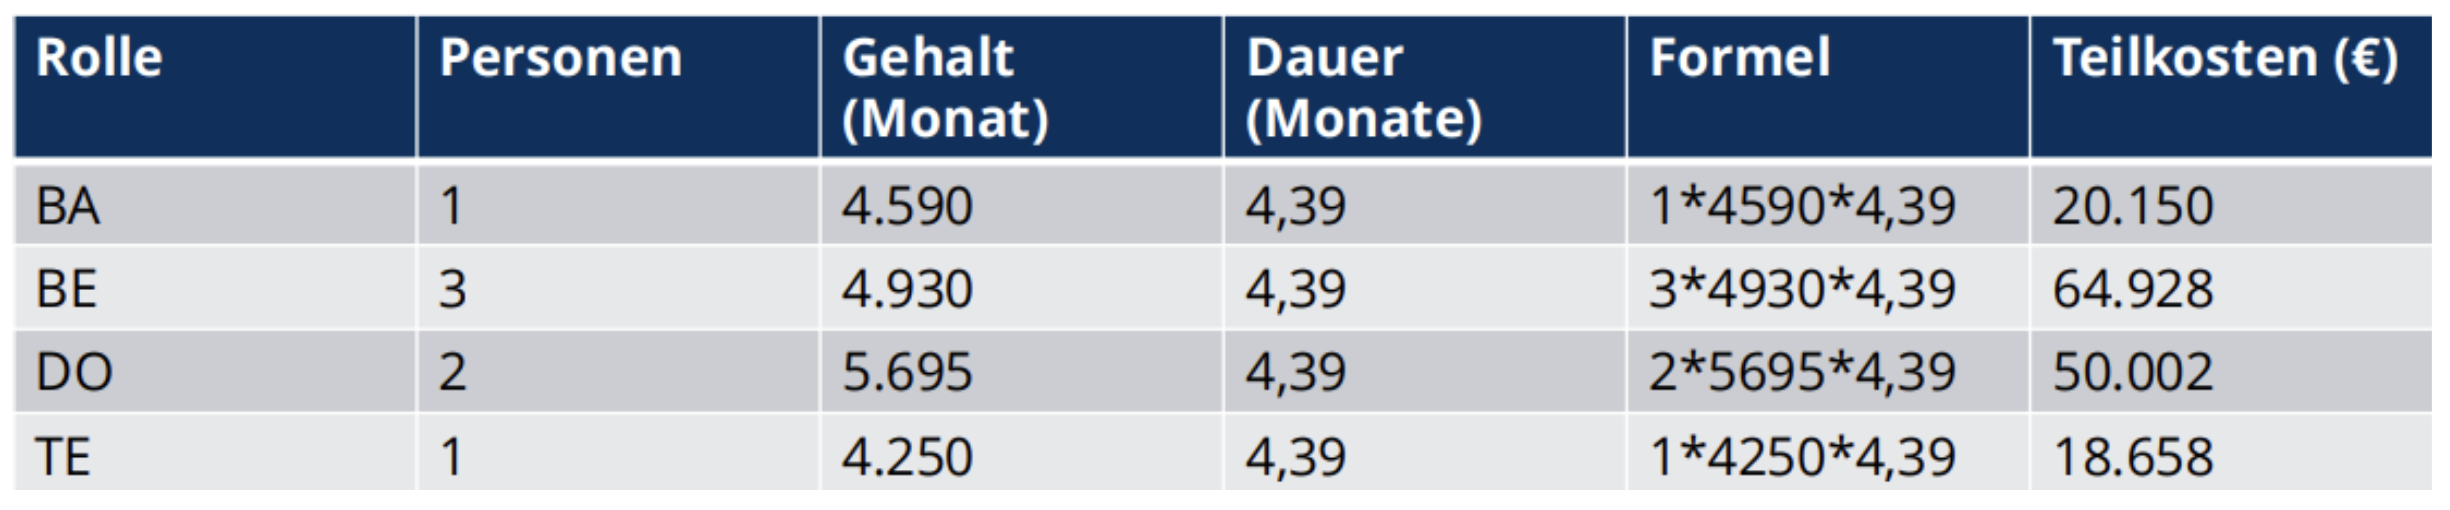
\includegraphics[width=0.9\textwidth]{fig/Kosten1.png}
	\caption{Personalkosten}
	\label{fig:personalkosten}
\end{figure}
Dabei entstehen Gesamtkosten von 153.738€. Eine vollständige Übersicht aller Arbeitspakete zeigt, dass die geplanten Personalkosten bei ca. 2.067.697€ liegen:

\begin{figure}[ht]
	\centering
	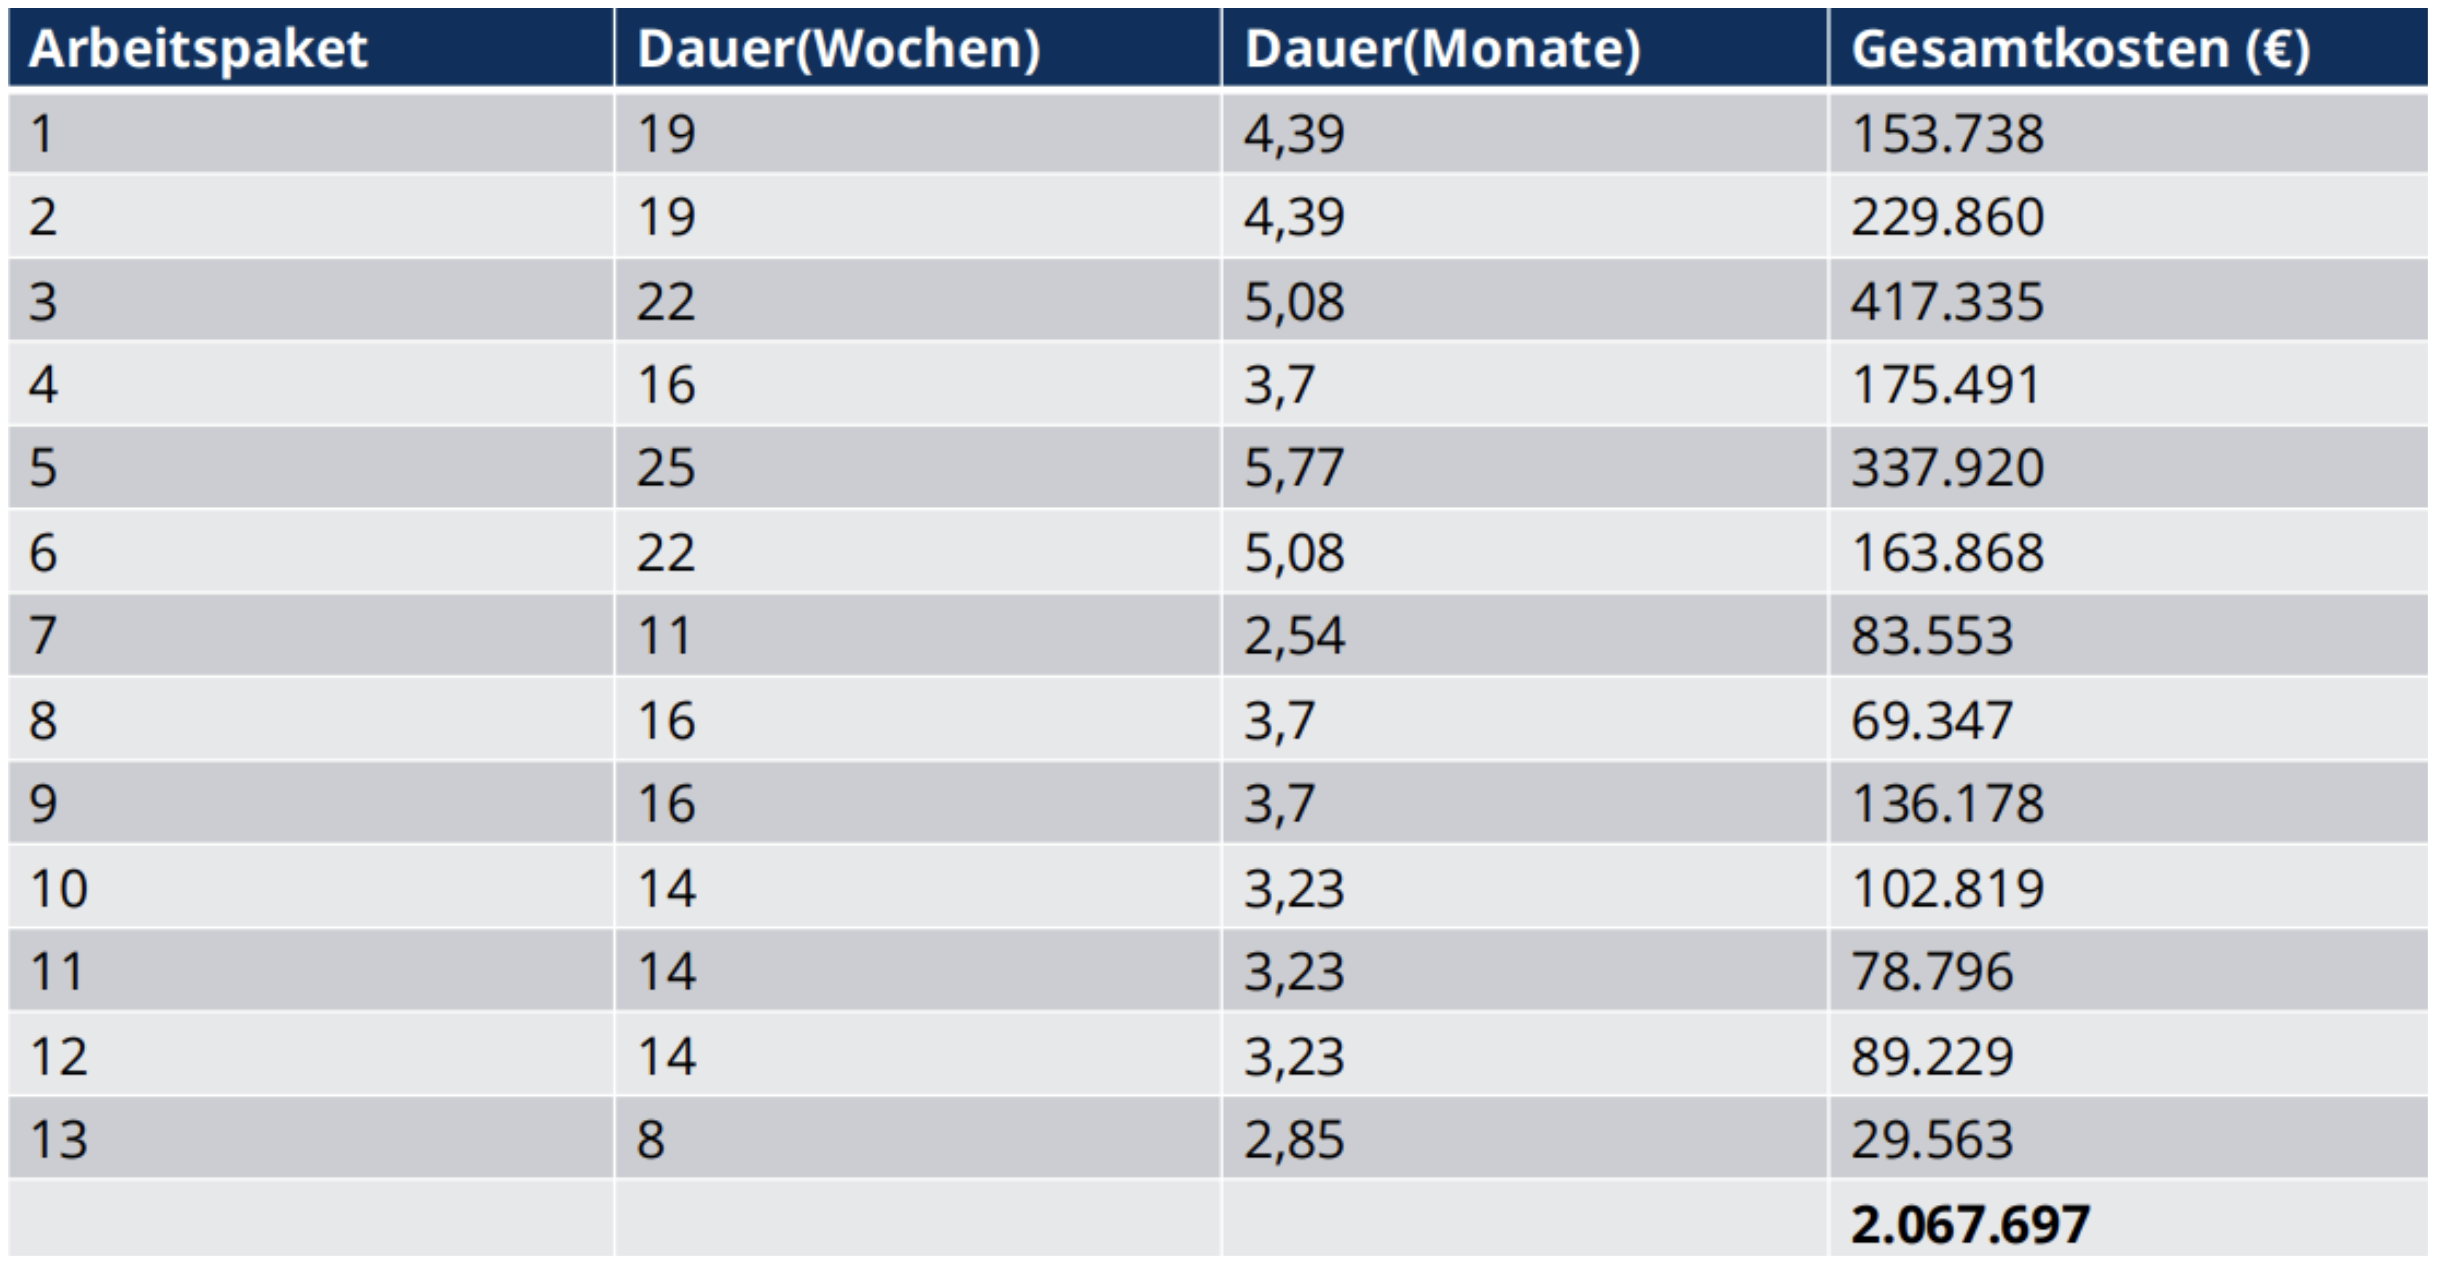
\includegraphics[width=0.9\textwidth]{fig/Kosten2.png}
	\caption{Gesamtkosten des Personals}
	\label{fig:personalkosten_gesammt}
\end{figure}
\pagebreak
Bei dieser Berechnung wird von einer Zeitauslastung von 100 \% ausgegangen. Diese ist jedoch nicht realistisch, da in den Arbeitspaketen bereits ein Puffer für Verzögerungen eingerechnet ist. 
Wird die realistischere Annahme von 75 \% des geplanten Zeitaufwands zugrunde gelegt, reduzieren sich die Kosten auf 1.551.209€, woraus ein Puffer von über 500.000€ entsteht. 

\section{Weitere Kosten}
Neben den Personalkosten fallen weitere projektbezogene Aufwendungen an, die in einmalige Fixkosten und laufende (variable) Kosten unterteilt werden können:
\\Einmalige Fixkosten:\\
Diese umfassen Anschaffungen, die nur zu Beginn des Projekts notwendig sind:
\begin{itemize}
	\item Server- und Backup-Systeme: 7000€
	\item Projektlaptops und Zubehör: 8000€
	\item Software: 76.000€
	\item Infrastruktur (Netzwerk, Sicherheit): 8.000€
	\item Testgeräte und Prototyping-Materialien: 10.000€
\end{itemize}
Die gesamten Fixkosten belaufen sich folglich auf ca. 109.000€.
\\Laufende (variable) Kosten:\\
Diese entstehen kontinuierlich während der Projektlaufzeit durch:
\begin{itemize}
	\item Personal (Ø pro Monat): ca. 43.000€
	\item Leasing Geräte/Hardware 1.000€
	\item Energiekosten: 800€ 
	\item Instandhaltungen Reparaturen: 600€
	\item Allg. Betriebskosten/Umlagen: 700€
	\item Konvertierung/Datenmigration: 1.000€
	\item Datenleitungen \& VPN: 500€
	\item Abschreibung technischer Geräte: 500€
	\item Miete Büroräume: 4.620€ (226m² Dresden)
	\item Lizenzkosten Cloverleaf ab 13. Monat: 5.000€ 
	\item Lizenzkosten IDE, JIRA, ... für 3 Jahre: ca. 10.000€
\end{itemize}
Laufende Kosten im ersten Jahr belaufen sich auf 615.468€, in den Jahren 2 und 3 jeweils auf 684.468€. 
Die Gesamtkosten für die Entwicklung belaufen sich damit auf \textbf{2.103.404€}. Darauf berechnen wir einen Gewinnaufschlag von 10 \%, also 210.000€. Zuzüglich Umsatzsteuer von 19 \% ergibt sich ein Endbetrag von \textbf{2.753.356€}, welcher unser Angebot ist.

